\documentclass[a4paper]{article}
\usepackage[utf8]{inputenc} % Skal passe til editorens indstillinger
\usepackage[english]{babel} % danske overskrifter


\newcommand{\name}{Carsten Nielsen, Eloy Parra Barrero,\\ Karla Burelo}
%\newcommand{\stnumber}{s123369, s123161, s123821}
\newcommand{\course}{INI 405 Neuromorphic Engineering~II}
\newcommand{\university}{University of Zürich}
\newcommand{\studyline}{Institute of Neuroinformatics}
\newcommand{\assignment}{Lab 7 Report}
\renewcommand{\date}{\today} %If another date, than that of today is desiered


% Palatino for rm and math | Helvetica for ss | Courier for tt
\usepackage{mathpazo} % math & rm
\linespread{1.05}        % Palatino needs more leading (space between lines)
\usepackage{palatino} % tt
\normalfont
\usepackage[T1]{fontenc}

\usepackage{graphicx}%allerese hentet % indsættelse af billeder
\usepackage{epstopdf} %Tilfj "--enable-write18" i argumentet for LaTex build. Dette vil konvertere .eps figurer til pdf-format
\graphicspath{{./picture/}} % stivej til bibliotek med figurer
\usepackage{subcaption} %Til gruppering af figurer
\usepackage{amsmath} %matpakke
\usepackage{amsfonts} %
\usepackage{amssymb} %
\usepackage{steinmetz} % flere matematik symboler
\usepackage{polynom} %for displaying polynom division
\usepackage{mathtools} % matematik - understøtter muligheden for at bruge \eqref{}
\usepackage{float}
\usepackage{placeins}
\usepackage{hhline}
\usepackage{rotating}

%
\usepackage[usenames,dvipsnames]{xcolor}
\usepackage[compact,explicit]{titlesec}% http://ctan.org/pkg/titlesec
%
\usepackage[europeanresistors]{circuitikz}


%---------%
%Easy edit%
%---------%

%Section formating. arg1 is supplied when making section
\newcommand\presectionnumber[1]{~~}
\newcommand\postsectionnumber[1]{}
\newcommand\midlesection[1]{#1}
\newcommand\sectionnum[1]{\arabic{#1}}
\newcommand\subsectionnum[1]{\arabic{#1}}
\newcommand\subsubsectionnum[1]{\alph{#1}}



%------------%
%setion setup%
%------------%
\renewcommand\thesection{Opgave~\sectionnum{section}} %pas p�, kun i matematik
\renewcommand\thesubsection{\thesection,~\subsectionnum{subsection}}
\definecolor{MagRed}{RGB}{190,40,15}
\definecolor{MathGreen}{RGB}{82,164,0}

\titleformat{\section}{\normalfont\sffamily\large\bfseries\color{MathGreen}}{}{0pt}{|\kern-0.15ex|\kern-0.15ex|\kern-0.15ex|\presectionnumber{#1}\sectionnum{section}\postsectionnumber{#1}\qquad\quad\midlesection{#1}\label{sec:\sectionnum{section}}}
\titleformat{\subsection}{\large\bfseries}{}{10pt}{\sectionnum{section}.\subsectionnum{subsection}~#1\label{sec:\sectionnum{section}.\subsectionnum{subsection}}}
%\titleformat{\subsubsection}[runin]{\itshape}{}{0pt}{\subsectionnum{subsection},\subsubsectionnum{subsection}~#1\label{sec:\sectionnum{section}.\subsectionnum{subsection}.\subsubsectionnum{subsubsection}}}
%\titleformat{\subsubsection}{\bfseries}{}{0pt}{\alph{subsection}.\arabic{subsubsection})\qquad\quad#1\label{\arabic{section}\alph{subsection}\arabic{subsubsection}}}
\titleformat{\subsubsection}{\bfseries}{}{0pt}{\arabic{subsubsection})\qquad\quad#1\label{\arabic{section}\alph{subsection}\arabic{subsubsection}}}

%----------%
%page setup%
%----------%
\textwidth = 400pt
\marginparwidth = 86pt
\hoffset = -25pt
\voffset= -30pt
\textheight = 670pt

%--------%
%hyperref%
%--------%
\newcommand{\HRule}{\rule{\linewidth}{0.5mm}}
\usepackage{fancyhdr}
\usepackage[plainpages=false,pdfpagelabels,pageanchor=false]{hyperref} % aktive links
\hypersetup{%
  pdfauthor={\name},
  pdftitle={\assignment},
  pdfsubject={\course} }
%\usepackage{memhfixc}% rettelser til hyperref

%-------------%
%Headder setup%
%-------------%
\fancyhf{} % tom header/footer
\fancyhfoffset{20pt}
\fancyhfoffset{20pt}
\fancyhead[OL]{\name}
\fancyhead[OC]{Date \\ \date}
\fancyhead[OR]{\university\\ \studyline}
\fancyfoot[FL]{}
\fancyfoot[FC]{\thepage}
\fancyfoot[FR]{}
\renewcommand{\headrulewidth}{0.4pt}
\renewcommand{\footrulewidth}{0.4pt}
\headsep = 35pt
\pagestyle{fancy}
 % style setup

%Listings%
\usepackage{listingsutf8}
\usepackage[framed,numbered]{matlab-prettifier}


%setup listings
\lstset{language=Matlab,
  extendedchars=true,
  language=Octave,                % the language of the code
  basicstyle=\ttfamily\footnotesize,           % the size of the fonts that are
  % used for the code
  numbers=left,                   % where to put the line-numbers
  numberstyle=\tiny\color{gray},  % the style that is used for the line-numbers
  stepnumber=2,                   % the step between two line-numbers. If it's 1, each line 
                                  % will be numbered
  numbersep=5pt,                  % how far the line-numbers are from the code
  backgroundcolor=\color{white},      % choose the background color. You must add \usepackage{color}
  showspaces=false,               % show spaces adding particular underscores
  showstringspaces=false,         % underline spaces within strings
  showtabs=false,                 % show tabs within strings adding particular underscores
  frame=single,                   % adds a frame around the code
  rulecolor=\color{black},        % if not set, the frame-color may be changed on line-breaks within not-black text (e.g. comments (green here))
  tabsize=4,                      % sets default tabsize to 2 spaces
  captionpos=b,                   % sets the caption-position to bottom
  breaklines=true,                % sets automatic line breaking
  breakatwhitespace=false,        % sets if automatic breaks should only happen at whitespace
  title=\lstname,                   % show the filename of files included with \lstinputlisting;
                                  % also try caption instead of title
  %keywordstyle=\color{blue},          % keyword style
  %commentstyle=\color{dkgreen},       % comment style
  %stringstyle=\color{mauve},         % string literal style
  escapeinside={\%*}{*)},            % if you want to add LaTeX within your code
  morekeywords={*,...},              % if you want to add more keywords to the set
  deletekeywords={...}              % if you want to delete keywords from the given language
}
\lstset{literate=
  {á}{{\'a}}1 {é}{{\'e}}1 {í}{{\'i}}1 {ó}{{\'o}}1 {ú}{{\'u}}1
  {Á}{{\'A}}1 {É}{{\'E}}1 {Í}{{\'I}}1 {Ó}{{\'O}}1 {Ú}{{\'U}}1
  {à}{{\`a}}1 {è}{{\`e}}1 {ì}{{\`i}}1 {ò}{{\`o}}1 {ù}{{\`u}}1
  {À}{{\`A}}1 {È}{{\'E}}1 {Ì}{{\`I}}1 {Ò}{{\`O}}1 {Ù}{{\`U}}1
  {ä}{{\"a}}1 {ë}{{\"e}}1 {ï}{{\"i}}1 {ö}{{\"o}}1 {ü}{{\"u}}1
  {Ä}{{\"A}}1 {Ë}{{\"E}}1 {Ï}{{\"I}}1 {Ö}{{\"O}}1 {Ü}{{\"U}}1
  {â}{{\^a}}1 {ê}{{\^e}}1 {î}{{\^i}}1 {ô}{{\^o}}1 {û}{{\^u}}1
  {Â}{{\^A}}1 {Ê}{{\^E}}1 {Î}{{\^I}}1 {Ô}{{\^O}}1 {Û}{{\^U}}1
  {œ}{{\oe}}1 {Œ}{{\OE}}1 {æ}{{\ae}}1 {Æ}{{\AE}}1 {ß}{{\ss}}1
  {ç}{{\c c}}1 {Ç}{{\c C}}1 {ø}{{\o}}1 {å}{{\r a}}1 {Å}{{\r A}}1
  {€}{{\EUR}}1 {£}{{\pounds}}1
}

 \lstloadlanguages{% Check Dokumentation for further languages ...
         %[Visual]Basic
         %Pascal
         %C
         %C++
         %XML
         %HTML
         %Java
         %VHDL
         Matlab
 }
 %Listings slut%









%Matematik hurtige ting
%fed
\renewcommand\vec[1]{\mathbf{#1}}
\newcommand\matr[3]{{}_{#2}\mathbf{#1}{}_{#3}}
\newcommand\facit[1]{\underline{\underline{#1}}}
%\renewcommand\d[3]{\frac{\mbox{d}^{#3}#1(#2)}{\mbox{d}#2^{#3}}}
%underline
%\renewcommand\vec[1]{\underline{#1}}
%\newcommand\matr[3]{{}_{#2}\underline{\underline{#1}}{}_{#3}}

\renewcommand\matrix[4]{ %{alignment}{to space}{from space}{matrix}
{\vphantom{\left[\begin{array}{#1}#4\end{array}\right]}}_{#2}\kern-0.5ex
\left[\begin{array}{#1}
#4
\end{array}\right]_{#3}
}
\newcommand\e[0]{\mbox{e}}
\newcommand\E[1]{\cdot 10^{#1}}
\newcommand\im[0]{i}

\newcommand\Jaco{\mbox{Jacobi}}
\newcommand\del[2]{\frac{\partial {#1}}{\partial {#2}}}
\newcommand\abs[1]{\left| {#1} \right|}
\newcommand\stdfig[4]{ %width,img,cap,lab
\begin{figure}[H]
\centering
\includegraphics[width={#1}\textwidth]{#2}
\caption{#3}
\label{#4}
\end{figure}
}
\newcommand\stdfignoscale[3]{ %img,cap,lab
\begin{figure}[H]
\centering
\includegraphics{#1}
\caption{#2}
\label{#3}
\end{figure}
}
\newcommand\diff{\dot}
\newcommand\ddiff{\ddot}
\newcommand\dddiff{\dddot}
\newcommand\ddddiff{\ddddot}






% How to make ref to books or urls in bib
%\citetitle[fx: page 1]{name of ref in bib}

\tikzset{rrail/.style={rground,yscale=-1}}
\begin{document}
\begin{titlepage}
\centering \parindent=0pt

\vspace*{\stretch{1}} \HRule\\[1cm]\Huge
\course\\[0.7cm]
\large \assignment\\[1cm]
\HRule\\[4cm]  
%\includegraphics[width=6cm]{picture}\\ Use this if you want a picture on the frontpage
\name\\
%\stnumber

\vspace*{\stretch{2}} \normalsize %
\begin{flushleft}

\date \end{flushleft}
\vspace*{\stretch{2}} \normalsize
\begin{flushright}
%\includegraphics[width=6cm]{./dtu.eps}\\
\end{flushright}
\end{titlepage}

\newpage
\setcounter{section}{1}
\begin{figure}
    \center
    \begin{subfigure}{0.3\textwidth}
        \center
        \begin{circuitikz} \draw
            (0,0) node[nmos] (n) {}
            (n.source) node[anchor=north] {S}
            (n.drain) node[anchor=south] {D}
            (n.gate) node[anchor=east] {G}
            (n.drain) to[short, i=$I_{ds}$] ++(0,-0.2)
        ;\end{circuitikz}
        \caption{}
    \end{subfigure}
    \begin{subfigure}{0.3\textwidth}
        \center
        \begin{circuitikz} \draw
            (0,0) node[pmos] (p) {}
            (p.source) node[anchor=south] {S}
            (p.drain) node[anchor=north] {D}
            (p.gate) node[anchor=east] {G}
            (p.source) to[short, i=$I_{ds}$] ++(0,-0.2)
        ;\end{circuitikz}
        \caption{}
    \end{subfigure}
    \caption{nFET (a) with gate (G), drain (D) and source (S), and a pFET (b) with the same terminals.}
    \label{fig:fets}
\end{figure}
\section{Transistor Operation in the Subthreshold Domain}
\subsection{(a) nFET drawing}
See Fig.~\ref{fig:fets}.
\subsection{(b) Subthreshold current expression}
The expression for the current from drain to source, \(I_{ds}\) in an NFET is 
\begin{equation*}
    I_{ds} = I_0e^{\frac{\kappa V_g}{U_T}}\left(e^{\frac{-V_s}{U_T}}-e^{\frac{-V_d}{U_T}}\right)
\end{equation*}
Which can be split up into the positive forward current 
\begin{equation*}
    I_f = I_0e^{\frac{\kappa V_g-V_s}{U_T}}
\end{equation*}
And negative reverse current
\begin{equation*}
    I_r = I_0e^{\frac{\kappa V_g - V_d}{U_T}}
\end{equation*}
\subsection{(c) Effects of drain and source voltages}
Decreasing the source voltage \(V_s\) has the effect of (i) increasing the forward current, (ii) but it has no effect on
the reverse current.

Conversely, decreasing the drain voltage \(V_d\) (i) does not affect the forward current, (ii) but it increases the reverse current.

\subsection{(d) Relative magnitudes of forward and reverse currents}
A transistor operating in subthreshold is in saturation when \(V_{ds}>4U_T\). Given that \(e^4 \simeq 55\), the relative magnitudes of 
the forward and reverse currents are (i) less than two orders of magnitude in the ohmic region and (ii) more than two orders of magnitude 
in saturation.

\subsection{(e) Approximate values of \(V_{ds}\)}
A transistor in subthreshold is in the ohmic region when \(V_{ds}<4U_T\) and in saturation when \(V_{ds}>4U_T\).

\subsection{(f) pFETs}
See Fig.~\ref{fig:fets} for the pFET drawing.

The expression for current through a pFET in subthreshold is
\begin{equation*}
    I_{ds} = I_0e^{\frac{\kappa (V_w-V_g)}{U_T}}\left(e^{\frac{(V_w-V_s}{U_T}}-e^{\frac{(V_w-V_d}{U_T}}\right)
\end{equation*}
Where \(V_w\) is the bulk voltage of the pFET transistor.

This can be broken up into a forward current
\begin{equation*}
    I_f = I_0e^{\frac{\kappa (V_w-V_g)-(V_w-V_s)}{U_T}}
\end{equation*}
And a reverse component
\begin{equation*}
    I_r = I_0e^{\frac{\kappa (V_w-V_g)-(V_w-V_d)}{U_T}}
\end{equation*}

\section{Linear Resistance Circuit}
\begin{figure}
    \center
    \begin{subfigure}{0.3\textwidth}
        \center
        \begin{circuitikz} \draw 
            (0,0) node[pmos, rotate=-90] (p) {}
            (p.B) node[anchor=north] {$M_1$}
            (p.source) node[anchor=west] {$V_2$}
            (p.drain) node[anchor=east] {$V_1$}
            (p.gate) node[anchor=south] {$V_b$}
            (p.drain) to[short,i=$I_{M1}$] ++(0.1,0)
        ;\end{circuitikz}
    \end{subfigure}
    \begin{subfigure}{0.3\textwidth}
        \center
        \begin{circuitikz} \draw
            (0,0) node[nmos] (m4) {}
            (m4.drain) to[short] ++(0,0.0) node[rrail] {}
            (m4.B) node[anchor=west] {$M_4$}
            (0,-2) node[nmos] (m3) {}
            (m3.B) node[anchor=west] {$M_3$}
            (m3.source) to[short, i=$I_b$] ++(0,-0.1) node[ground] {}
            (m3.drain) -- (m4.source) -- ++(0.5,0) node[anchor=west] {$V_b$}
            (m4.gate) node[anchor=east] {$V_1$}
            (m3.gate) node[anchor=east] {$V_m$}
        ;\end{circuitikz}
    \end{subfigure}
    \caption{Linear resistance circuit.}
    \label{fig:linres}
\end{figure}

\subsection{(a) Expression for current through M1 and M4}
The common mode voltage \(V_{cm}\) is the average of the inputs.
\begin{equation*}
    V_{cm} = \frac{V_1+V_2}{2}
\end{equation*}
And the differential voltage is 
\begin{equation*}
    \Delta V = V_1 - V_2
\end{equation*}
From this it follows that
\begin{equation*}
    V_1 = V_{cm} + \frac{\Delta V}{2} \quad , \quad V_2 = V_{cm} - \frac{\Delta V}{2}
\end{equation*}
And therefore the expression for the current through M1 can be rewritten as
\begin{equation}
    I_{M1} = I_0e^{\frac{\kappa (V_w - V_b) - (V_w - V_{cm})}{U_T}}\left(e^{\frac{\Delta V}{2U_T}}-e^{\frac{-\Delta V}{2U_T}}\right)
    \label{eq:IM1}
\end{equation}
For positive current in the direction noted in Fig.~\ref{fig:linres}.

The current through M4 is \(I_b\) and given by 
\begin{equation*}
    I_b = I_0e^{\frac{\kappa V_1 - V_b}{U_T}}
\end{equation*}
Assuming that M4 is in subthreshold saturation.

\subsection{(b) M1 current continued}
Substituting 
\begin{equation*}
    V_b = \kappa V_1 - U_T\ln\left(\frac{I_b}{I_0}\right) = \kappa \left( V_{cm} + \frac{\Delta V}{2} \right) - U_T\ln\left(\frac{I_b}{I_0}\right)
\end{equation*}
In~\ref{eq:IM1} yields
\begin{equation*}
    I_{M1} = I_0e^{\frac{\kappa (V_w - \kappa \left(V_{cm}+\frac{\Delta V}{2}\right) + U_T\ln\left(\frac{I_b}{I_0}\right)) - (V_w - V_{cm})}{U_T}}\left(e^{\frac{\Delta V}{2U_T}}-e^{\frac{-\Delta V}{2U_T}}\right)
\end{equation*}
Which reduces to
\begin{equation*}
    I_{M1} = I_b^\kappa e^{\frac{\kappa (V_w - \kappa \left(V_{cm}+\frac{\Delta V}{2}\right)) - (V_w - V_{cm})}{U_T}}\left(e^{\frac{\Delta V}{2U_T}}-e^{\frac{-\Delta V}{2U_T}}\right)
\end{equation*}
\begin{figure}
    \center
    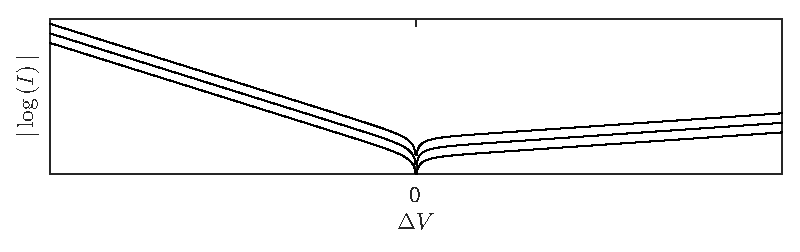
\includegraphics{matlabtimes.eps}
    \caption{Resistive element current versus \(\Delta V\) in arbitrary units. The curve moves upwards for increasing \(I_b\)}
    \label{fig:absI}
\end{figure}

Fig.~\ref{fig:absI} shows how the current behaves as a function of \(\Delta V\). The slope is smaller for positive differential voltages
because the gate voltage of the pFET transistor in the resistive element depends on \(\Delta V\), and higher gate voltages result in 
lower currents.
\end{document}
